Des données transmissent en utilisant le protocole IPv4 sont encapsulées dans un message que
l'on appelle un paquet IPv4. Ces paquets sont consitué d'un entête suivis des données à transmettre.

% Mossi
\subsection{Adresse IPv4}

L'entête contient des informations essentielles pour la transmission d'un paquet, notamment les
adresses source et destination.

Une adresse IP sert à identifier une machine (et plus précisement une des interfaces de cette machine)
dans un réseau particulié.
Comme nous le verrons plus tard cet identifiant unique permet de désigner à la fois un
réseau et une machine précise au sein de ce réseau.
Une adresse est codé sur 32 bits ce qui permet de coder 2\^32 soit 4294967296 adresses différentes.
Par convention on peut représenter une adresse IPv4 comme une suite de 4 nombres décimaux séparés par des points,
chacun traduisant un octet. Cette représentation a contribuée à simplifier l'utilisation et la manipulation
des adresses.
Comme chaque nombre représente un octet, les valeurs de celui-ci sont comprises entre 0 et 255.

\vspace{1cm}
Exemple: adresse à valeur décimale: 212.217.0.1 => correspond sous sa forme
binaire à: 11010100.11011001.00000000.00000001
\vspace{1cm}

\subsubsection{Notion de NET ID et HOST ID}
Une adresse IPv4, en tant qu'inditifiant d'une machine dans un réseau, contient deux informations:
une première partie qui identifie le réseau appellé NET ID (les bits de poids fort), une seconde qui identifie l’hôte appeler host-ID (les bits de poids faible).
Les machines qui se trouvent donc sur le même réseau partage le même NET ID pour leur adresse.

La longueur de ces deux parties est variable: la taille du HOST ID dépend de la taille du NET ID. Pour représenter la longueur de ces différentes parties on a introduit la notion de masque

\subsubsection{Masque de réseau}

Le masque sert à représenter la scission entre le NET ID et le HOST ID.
Il est codé sur 32 bits et adopte la même représentation qu'une adresse IP, à savoir
4 nombres décimaux séparé par des points.
La position des bits à 1 dans le masque corresponde à la position des bits définissant le NET ID dans l'adresse IP.
Pour obtenir les bits du NET ID il suffit de faire un ET logique entre l'adresse et son masque. Tous les autres bits (donc les bits à 0)
feront donc partie du HOST ID.
Les bits à 1 sont contiguës et commencent au bit de poids fort: le nombre de bit à 1 dans le masque, donne
le nombre de bit faisant partie du NET ID en partant du bit de poids fort dans l'adresse.

En conséquence plus le nombre de bit à 1 dans le masque est grand, plus le NET ID sera grand, et plus le HOST ID sera petit, car il restera moins de bit pour définir le HOST ID (la somme des deux devant évidemment faire 32 bits).

\begin{center}
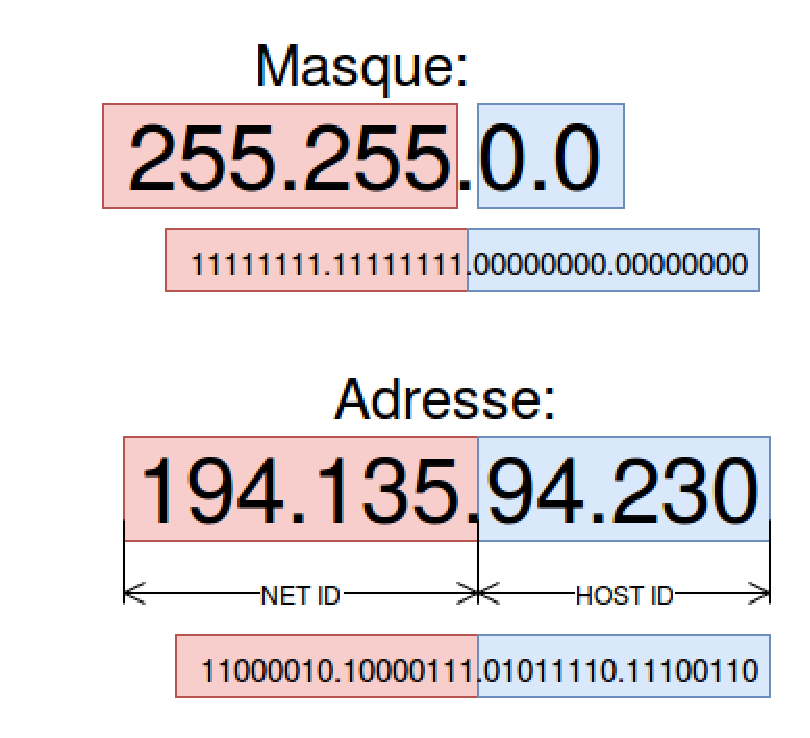
\includegraphics[width=7cm]{./pics/maskipv4.eps}
\end{center}

//TODO exemple
//TODO exemple invalide

\subsubsection{Classes d'adresse IP}
Historiquement les classes d'adresse IP correspondaient à une plages d'adresses avec un masque figer pour une classe donnée.
Ce système permettait de déduire le masque en fonction
de l'adresse IP étant donné que chaque classe avait son masque défini de manière standard.
Il fut décrit dans le RFC 791\cite{url-RFC-791}.

//TODO tableau classe

A partir de ce tableau nous pouvons voir qu'il suffit de regarder les 4 bits de
poids fort pour déduire à quelle classe appartient une adresse.  Par exemple si
une machine à pour adresse 152.123.87.45 on sait en regardant les 4 premiers
bits que cette adresse fait partie de la classe B (car l'adresse commence par
10). De là, la machine n'a pas besoin de masque en plus car elle sait que le
masque correspondant un adresse de classe B est 255.255.0.0 .

Ce système permet donc d'adresser de nombreux réseaux avec un nombre de machine
variable en fonction de la classe, et tout cela sans avoir besoin de
communiquer ou de paramétrer un masque; celui-ci étant normalisé pour chaque
classe.  Cependant il a un gros inconvénient, étant donné que les masques sont
figé, un réseau peux ne peux pas utiliser une partie plus ou moins importante
de ses adresses. Par exemple si un réseau contient 500 machines, il ne peux pas
utiliser d'adresse de classe A étant donné que celle-ci ne permettent d'avoir
que des réseaux de 254 machines maximum. Il va donc falloir utiliser des
adresses de classe B minimum, car elles permettent d'adresser 65534 machines au
sein d'un réseau. Nous pouvons donc utiliser 500 adresses sur les 65534
disponible, mais le reste sera "perdu".  Ce système était simpliste mais
n'était pas utilisable sur le long terme car il "gache" des adresses en
n'utilisant pas tout son espace d'adressage.


\subsubsection{CIDR}

Aujourd'hui le système le plus utilisé est CIDR (Classless Inter-Domain
Routing) remplace le système de classe d'adresse. CIDR permet de créer des
masque beaucoup plus fin, étant donné qu'on n'est plus limité à des masque de
réseau fixe, on peut ajuster le masque pour avoir le nombre de machine
adressable dans un réseau le plus proche possible du nombre de machine que l'on
souhaite adressé.  Cela permet de limiter les pertes en adresse inutilisé, si
la plage est correctement découpée.  On peut donc créer des masques à la
séparation entre le NET ID et le HOST ID se trouve n'importe où, même en plein
milieu des octets (ce qui était impossible avec les classes d'adresse), ce qui
apporte une plus grande fléxibilité.  Cela permet aussi de créer une hiérarchie
dans une plage d'adresse réseau qui serait découper en plusieurs réseaux
"fils", et cela permet notamment, avec cette hierarchie, de réduire la table de
routage des routeur.  De là est né une nouvelle notation des masques: on écrit
le nombre de bit à 1 dans le masque à la suite de l'adresse IP et séparé par un
slash.







\subsubsection{Types d'adresses}
La variete des exigence en matiere de reseaux a donne lieu a une progressive
classification des adresses selon des roles bien precis.  En effet pas toutes
les adresses IPv4 ont la meme signification: a certain adresses (ou plages
d'adresses) ont ete attribue par convention des fonctions ou caracteristiques
particuliers.  Dans la suite de cette partie on analysera les adresses IP sous
trois aspects differants: on classifiera d'abord les adresses par leur portee, 
puis on introduira le concept d'adresse publique et adresse prive, enfin
on parlera des fonctions speciales qui ont ete assigne a certaines adresses.


\paragraph{Porte des adresses}

%TODO portee d'un adresse: broadcast, multicast, anycast unicast%

\paragraph{Adresses publiques et adresses prive}

%Note: private --> 10.0.0.0/8, 172.16.0.0/12 192.168.0.0/16

\paragraph{Adresses speciales}
L'assignation d'un usage speciale a une adresse IP deculait de l'emergence
%TODO (apparition??) 
d'une nouvelle necessite dans le domaine des reseaux; c'est pour
ca que jusq'avant les annes 2002, l'attribution des roles speciaux des adresses
IPv4 ete distribue dans divers document, dont chaqun a propos d'une
problematique en particuliere. Le RFC3330 est un des premiers document a
rassembler les classification des adresses IPv4 selon leur role et signification.

%TODO lien%


\begin{description}
\item[0.0.0.0/8]
Cette plage d'adresses indique la machine courante dans la reseau courante.
Les adresses dans cette plage sont notement utilise dans certain protocoles de
configuration comme adresses source, lorsque une machine n'a pas encore etabli
son adresse effective.
%RFC 1122 %

\item[127.0.0.0/8]
Un adresse appartenent a cet bloque est denommes adresse de {\it loopback}.  Un
paquet envoye vers un tel adresse returne directement l'expediteur, sans sortir
du contexte de la machine emettrice. Parmi les adresses de cette plage,
127.0.0.1 est celui utilise le plus frequent\footnote{Comme le indique
le RFC 1122, certaines implementations de l'adresse de {\it loopback} se
limitent a utiliser le bloque 127.0.0.1/32, ce qui se traduit en utiliser juste
l'adresse 127.0.0.1 .}: dans plusieurs contextes cet adresses est referencee par
l'alias "{\it localhost}".\footnote{La correpondence entre le nom {\it localhost} et
l'adresse 127.0.0.1 est generalement mise en place par le systeme d'exploitation.
Dans les systemes de type UNIX une entree reliant ces deux entites est generalement
present dans le fichier "/etc/hosts".}
Un adresse de {\it loopback} n'a pas de sens au dehors
d'un host, pour cette raison normalement il ne devrait pas apparaitre dans la
reseau a aucun moment.

%RFC 1122 %

\item[169.254.0.0/16]
Cet plage d'adresses a ete designe comme contenant les adresses qu'on appelle
de {\it lien local}.  Les adresses dit de {\it lien local} sont utilise lorsque
une machine n'a aucun moyen d'obtenir un adresse IP (par example par le biais
d'un serveur DHCP ou simplement avec une configuration manuelle).  L'obtention
d'un adresse de {\it lien local} c'est fait de facon automatique a travers un
processus de autoconfiguration souvent appelle avec l'acronyme APIPA ({\it
Automatic Private Internet Protocol Addressing}) ou avec le nom IPv4LL.  Le
fonctionnement du processus APIPA (decrit dans le RFC 3927) est assez complexe
dans ses detailes et entraine l'utilisation de certaines fonctionnalites du
protocole ARP (qu'on traitera plus en detail dans la section %TODO \ref{sec:suiteproc} % )
.Il peut etre syntetizee dans ses grandes lignes par la demarche suivante:

\begin{description}
\item[Selection de l'adresse]
La machine choisit aleatoirement
    \footnote{Il est conseille de utiliser l'adresse MAC de l'interface en question
    pour generer l'adresse de {\it lien local} pour qu'il ait une plus forte chance
    qu'il soit unique dans le reseau.} 
un adresse appartenant a la plage 169.254.0.0/16

\item[Sondage sur l'adresse]
Une fois selectionne un adresse, il faut s'assurer que le meme adresse ne soit
pas deja utilise par d'autres machines dans la reseau. Dans ce but la machine
pose la question a toutes les autres machine de le reseau au moyen d'un ou plusieurs messages
en brodcast et attend une reponse pendant un certain intervalle de temp\footnote{
Des precautions sont prises pour eviter les conflits genere par plusieurs
machines qui effectuant simultanement cette action pour le meme adresse,
notament: des intervals de temps aleatoires entre l'envoi des messages, la mise
en place d'un ecoute active des autres messages pendat le temp de l'enquete.}
Le manque de reponse indique que l'adresse est bien unique. Si l'adresse n'est
pas unique il faudrait en choisir un outre.

\item[Annonciation de l'adresse]
A ce poit la machine peut comunniquer aux autres machines l'adresse qu'il
vient de reserver.

\end{description}



Cet processus est base sur le concept de {\it Zeroconf}: il permet la mise en
place d'un reseau IPv4 sans aucune configuration. Ce type de systeme,
C'est aussi grace a ce gendre de systemes, que on 
pourrait syntetiser par le devise %TODO slogan??  
"plug and play", que le concept de Networking (et avec lui Internet) a pu se
diffuser assez rapidement: grace a APIPA une reseau IPv4 peut etre facilement
mise an place sans le besoin de aucune connaissances techniques.\\

La plage d'adresses 169.254.0.0/16, designe une plage d'adresses prive: les
adresses de type {\it lien local} ne sont donc pas attaignables au dehors de
leur reseau de definition. 
Cet plage d'adresses pose  par contre des limites par rapport aux autres
plages d'adresses prive car, a difference des autres, il ne peut pas etre
divise en sous reseux\footnote{Ce qui est assez logique si on considere que
le processus d'obtention d'un adresse de {\it lien local} (APIPA) utilise
les liens "physiques" entres les machines pour communiquer, et il ne peut
pas considerer aucune notion de sous-reseau.}
: en effet un packet destine a un adresse de {\it lien local} ne doit pas etre
retrasmis par un host intermediaire.\footnote{Dans ls paquets destine
a un adresse de {\it lien local} le champ TTL est de norme mis a 1
pour empecher des forwarding.}

\item[192.88.99.0/24]
Les adresses appartenant a cet bloque designant des routeurs 
fournissant un service du type {\it 6to4}. Cet type de service
permet de relier des reseau IPv4 avec des reseau IPv6.
Les adresses dans cette place sont traite comme etant des adresses
de type {\it anycast}.


\end{description}




------------------------------------------
Alors on vient de voir que les adresses IP privées sont utilisable uniquement
sur des réseaux locaux, tandis qu’il y a des adresses IP qui ne sont utilisées
uniquement que sur internet donc nous pouvons en déduir que c’est les adresses
IP publiques non utilisable dans un réseau local. Les routeurs (par exemple:
votre box) ont une adresse IP publique du côté d’internet, ce qui permet de
rendre votre box visible sur internet (elle répondra certainement au ping). De
plus, au moment de vos connexion sur un site web vous utilisez l’adresse
publique du serveur web. De ce fait une adresse IP publique est unique dans le
monde, ce qui n’est pas le cas dans le systèmes d’adressage des adresses IP
privées qui doivent être unique seulement dans un même réseau local mais pas au
niveau planétaire étant donné que ces adresses ne peuvent pas être routées sur
internet. Une adresse IP publique est soit acheté ou fournie par la FAI.  Les
IP publiques représentent toutes les adresses IP des classes A, B et C qui ne
font pas partie de la plage d’adresses privées de ces classes ou des exceptions
de la classe A (voir Adresse non utilisé ci-dessus).


\subsubsection{Les classes d’adresses}
Au début de la création de IPV4, maintes groupes d’adresses ont été définis
pour faciliter le routage (ou cheminement) des paquets. Structurée en 5 classes
(A,B,C,D,E) selon la valeur du première octet.

%TODO images classes %
%TODO tableau recapitulatif %

De ce fait on remarque une distribution de l’espace d’adressage selon laquelle
la classe A possède 50\% l’espace et soit 25\% pour la classe B, 12,5\% classe
C et 6,25\% pour D \& E. on peut en-déduire une mauvaise répartition de cette
espace d’adressage. 

%--------------------------------------
Les classes A, B et C ont chacune une correspondance de plage
d’adresses IP privées à l’intérieur de la plage globale qui a été définie par
la RFC 1918. Mais l’utilisation  de celui-ci pour inter-connecter des réseau
géante (entreprise) avec des espaces adressage qui se chevauche peut causer des
problèmes. Une adresse IP privées est librement paramétrée par l’administrateur
du réseau local.
Les adresses privées de la classe A: 10.0.0.0 à 10.255.255.255\\
Les adresses privées de la classe B: 172.16.0.0 à 172.31.255.255\\
Les adresses privées de la classe C: 192.168.1.0 à 192.168.255.255\\


\textbf{Remarque:}
De ce fait on distingue deux adresses particulières parmi tout ceux possible,
qui ne doivent jamais être attribué à des machines:

     les bits Host-ID sont à 0 : adresse attribue qu’à un réseau.
Exemple: 192.168.10.0 / 255.255.255.0 = 192.168.10.00000000

    les bits Host-ID sont à 1 : c’est un adresse de  diffusion (broadcast),
Exemple: 172.27.255.255 / 255.255.0.0 = 172.27.1111111.11111111

Donc nous pouvons en déduire que parmi tout les adresses assignable, ces
derniers sont des adresses interdites.



\subsubsection{Adresses non utilisées}
il existe des adresses non utilisable comme adresse IP pour une machine:\\
les adresses réseaux: qui correspond aux adresses qui ont tous les bits de
leur partie hostid à zéro(0);\\
les adresses de diffusion (broadcast): qui correspond aux adresses qui ont
tous les bits de leur partie hostid à un(1)\\
0.0.0.0: utilise par différentes services (table de routage, DHCP) et possède
souvent une signification particulières. \\
127.X.X.X: désigne l’ordinateur lui-même ou dite adresse de bouclage
(lookback), 127.0.0.1 pour le localhost\\
> à 223.255.255.255: pour le multicast et la recherche.\\


